\documentclass[aspectratio=169, 10pt]{beamer}

\usetheme[progressbar=frametitle]{metropolis}
\usepackage{graphicx}
\usepackage{booktabs}
\usepackage{tikz}
\usepackage{hyperref}
\usepackage{fontawesome5}

\title{Retak.id}
\subtitle{Deteksi Dini Retakan Tanah Longsor \\ berbasis Crowdsourcing \& Edge AI}
\author{Jaweed \& Tim}
\date{IYREF 2026 — Semi-Final}
\titlegraphic{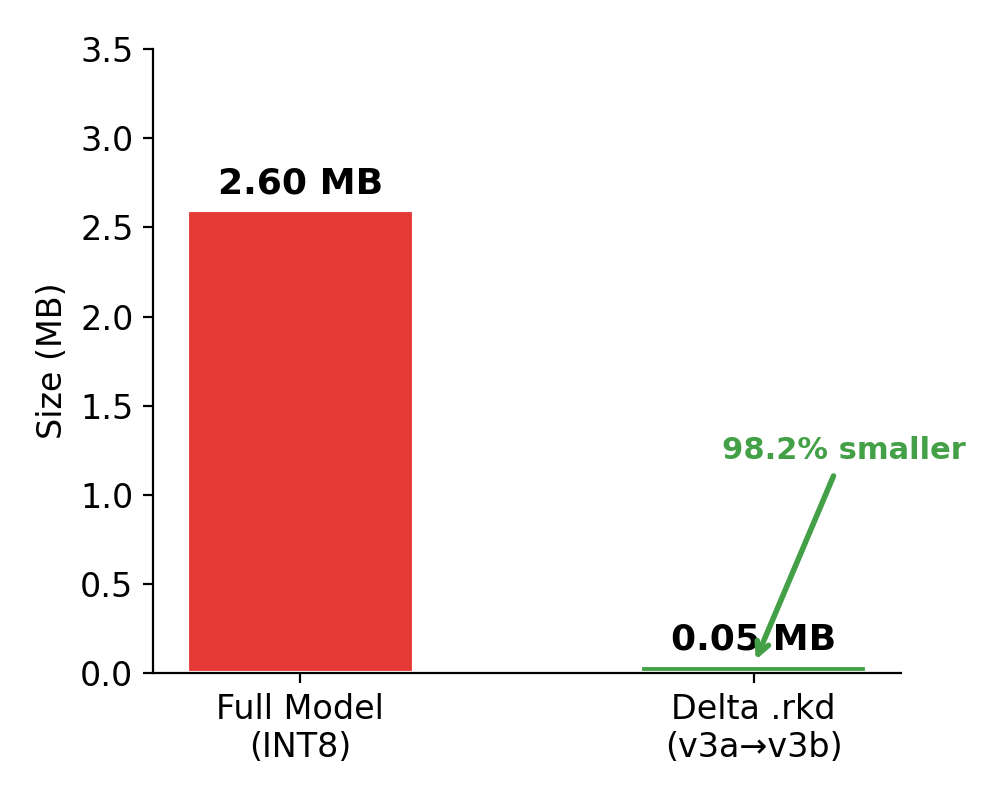
\includegraphics[height=0.8cm]{charts/model_size.png}}

\hypersetup{
  colorlinks=true, linkcolor=white, urlcolor=blue!70!white,
}

\begin{document}

% ── Slide 1: Cover ──
\maketitle

% ── Slide 2: Problem ──
\begin{frame}{Masalah}
  \textbf{Ancaman longsor laten}: 14 dari 24 desa di Jenangan, Ponorogo berada di \\ zona kerentanan tanah bergerak.
  \vspace{0.5cm}

  \begin{columns}[T]
    \column{0.48\textwidth}
    \textbf{Tantangan:}
    \begin{itemize}
      \item Tidak ada sistem peringatan dini berbasis visual
      \item Warga baru tahu kalo longsor sudah terjadi
      \item Ahli geologi terbatas, tidak bisa monitor 24/7
    \end{itemize}

    \column{0.48\textwidth}
    \textbf{Dampak:}
    \begin{itemize}
      \item Evakuasi terlambat
      \item Kerugian harta benda
      \item Risiko korban jiwa tiap musim hujan
    \end{itemize}
  \end{columns}
\end{frame}

% ── Slide 3: Solution ──
\begin{frame}{Solusi}
  \textbf{Crowdsourcing + Edge AI:} Warga cukup foto retakan tanah dari HP --- \\ ML model menganalisis langsung di perangkat, tanpa perlu cloud.
  \vspace{0.3cm}

  \begin{columns}[T]
    \column{0.48\textwidth}
    \centering
    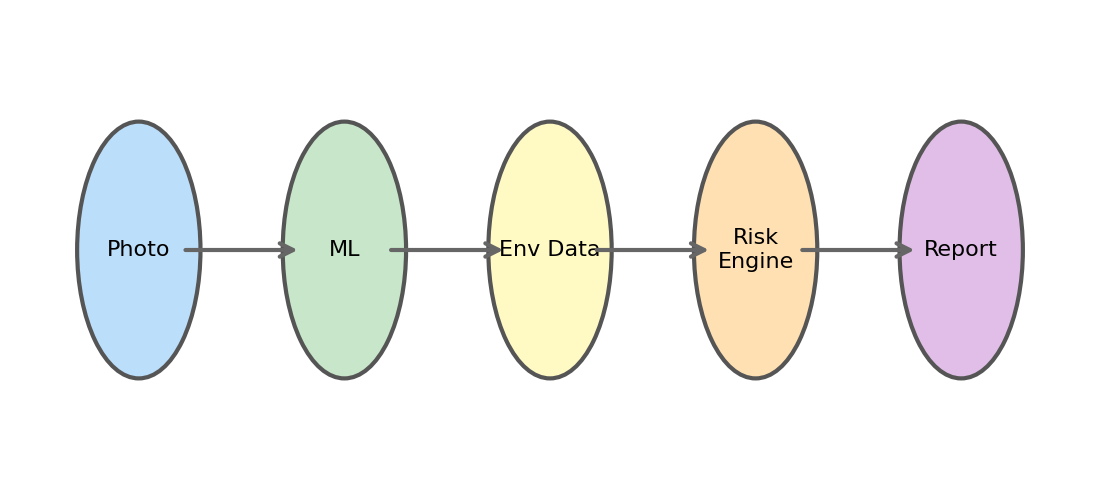
\includegraphics[width=\textwidth]{charts/bot_flow.png}

    \column{0.48\textwidth}
    \centering
    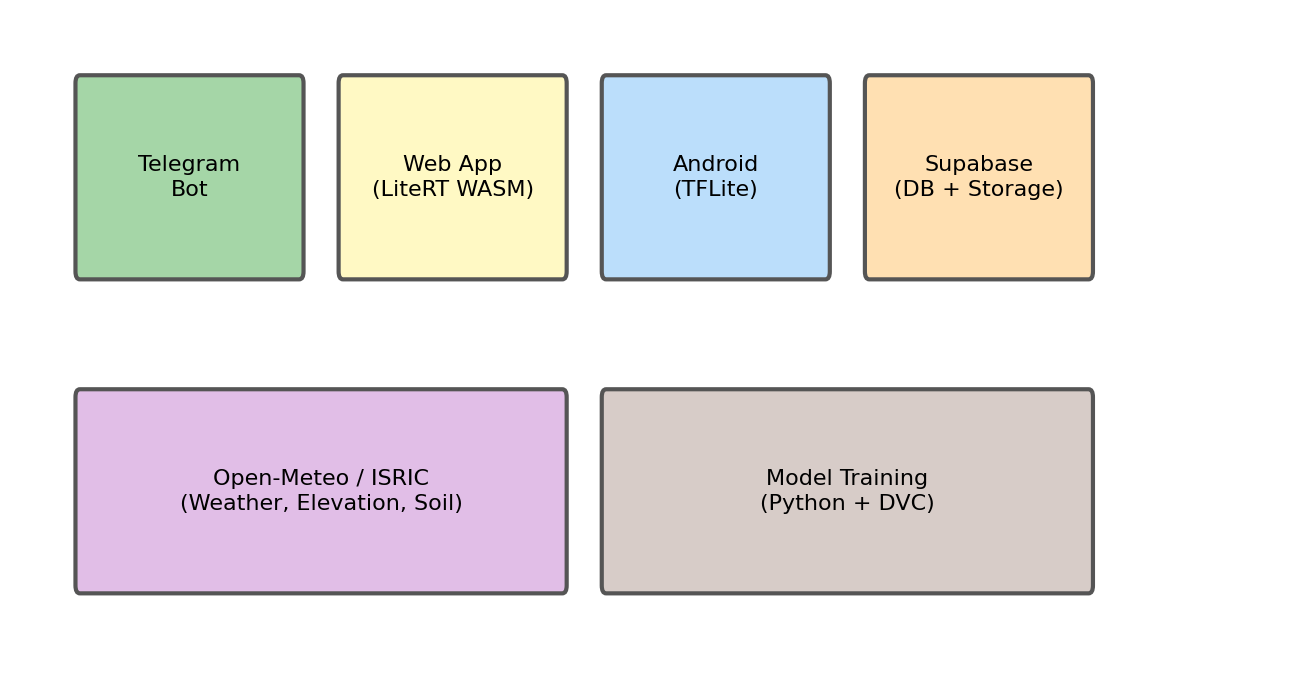
\includegraphics[width=\textwidth]{charts/architecture.png}
  \end{columns}
\end{frame}

% ── Slide 4: Edge Inference ──
\begin{frame}{Edge Inference --- Satu Model, Dua Platform}
  \begin{columns}[T]
    \column{0.48\textwidth}
    \textbf{Android (Kotlin)}
    \begin{itemize}
      \item TFLite Interpreter 2.16.1 (4 thread)
      \item Resize bilinear 224×224
      \item Threshold: 40\% $\rightarrow$ AMAN
      \item Delta OTA model updates
    \end{itemize}
    \vspace{0.3cm}
    \textbf{Web App (TypeScript)}
    \begin{itemize}
      \item LiteRT WASM @litertjs/core
      \item Resize high-quality 224×224
      \item Threshold: 50\% $\rightarrow$ TIDAK PASTI
      \item PWA cache offline-ready
    \end{itemize}

    \column{0.48\textwidth}
    \centering
    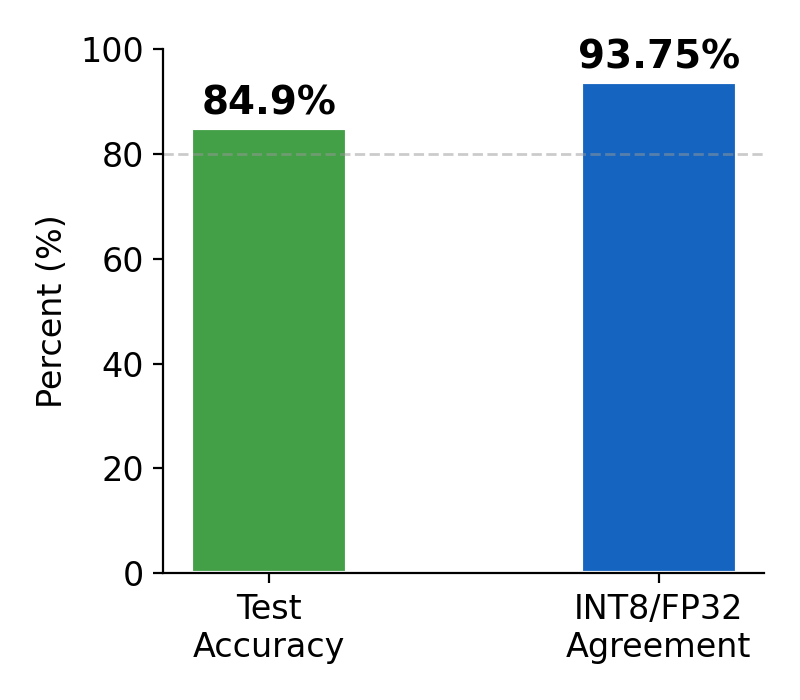
\includegraphics[width=\textwidth]{charts/accuracy.png}
    \vspace{0.2cm}

    \textbf{ Identical pipeline:}
    \begin{itemize}
      \item Model: \texttt{retak\_mobilenetv2.tflite}
      \item Input: 224×224 RGB uint8 [0,255]
      \item Softmax: $\frac{\exp(x_i - \max)}{\sum \exp(x_j - \max)}$
    \end{itemize}
  \end{columns}
\end{frame}

% ── Slide 5: ML Model ──
\begin{frame}{Model Machine Learning}
  \begin{columns}[T]
    \column{0.45\textwidth}
    \begin{tabular}{ll}
      \toprule
      \textbf{Parameter} & \textbf{Value} \\
      \midrule
      Architecture & MobileNetV2 \\
      Input & 224×224×3 uint8 \\
      Parameters & $\sim$2.26M \\
      Quantization & INT8 PTQ \\
      File size & \textbf{2.6 MB} \\
      Classes & 3 (AMAN, WASPADA, BAHAYA) \\
      \bottomrule
    \end{tabular}
    \vspace{0.3cm}

    \textbf{Accuracy:} 84.9\% test accuracy \\
    \textbf{FP32 agreement:} 93.75\%

    \column{0.52\textwidth}
    \centering
    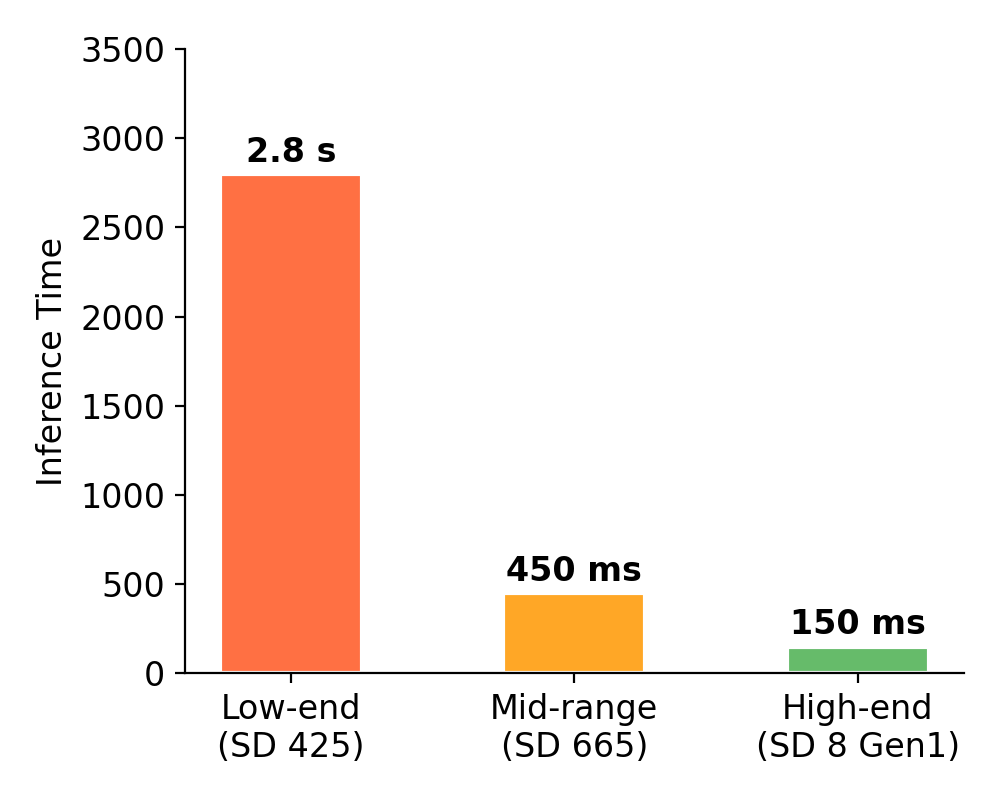
\includegraphics[width=\textwidth]{charts/inference_perf.png}
  \end{columns}
\end{frame}

% ── Slide 6: MultiFactor Risk ──
\begin{frame}{Multi-Factor Risk Engine}
  ML saja tidak cukup --- risiko longsor dipengaruhi banyak faktor:

  \vspace{0.3cm}
  \begin{columns}[T]
    \column{0.45\textwidth}
    \centering
    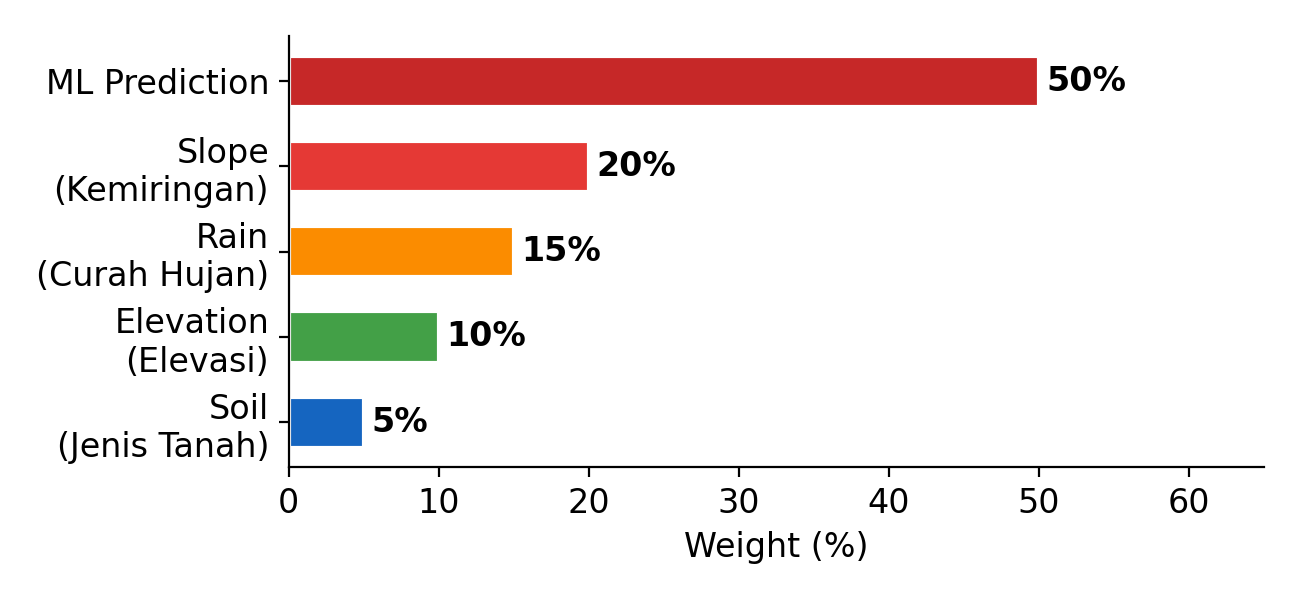
\includegraphics[width=\textwidth]{charts/risk_weights.png}

    \column{0.52\textwidth}
    \textbf{Bobot:}
    \begin{itemize}
      \item ML Prediction: \textbf{50\%}
      \item Slope: \textbf{20\%} --- kemiringan lereng
      \item Rain: \textbf{15\%} --- curah hujan real-time
      \item Elevation: \textbf{10\%} --- ketinggian
      \item Soil: \textbf{5\%} --- jenis tanah
    \end{itemize}
    \vspace{0.2cm}
    \textbf{Graceful degradation:} Jika API lingkungan gagal, bobot didistribusi ulang ke faktor lain.
  \end{columns}
\end{frame}

% ── Slide 7: Delta OTA ──
\begin{frame}{Delta OTA --- 98\% Bandwidth Savings}
  \textbf{Masalah:} 10.000 user $\times$ 2.6 MB = 26 GB bandwidth per rilis model.

  \vspace{0.2cm}
  \begin{columns}[T]
    \column{0.48\textwidth}
    \textbf{Solusi:} Byte-level delta patch
    \begin{itemize}
      \item Hanya kirim byte yang berubah antar versi
      \item Format .rkd: gzip + region patches
      \item Gates: savings > 50\%, size match, TFLite validation
    \end{itemize}

    \vspace{0.2cm}
    \textbf{Real result:}
    \begin{tabular}{ll}
      \toprule
      Full model & 2.6 MB \\
      Delta .rkd & \textbf{47 KB} \\
      Savings & \textbf{98.2\%} \\
      \bottomrule
    \end{tabular}

    \column{0.48\textwidth}
    \centering
    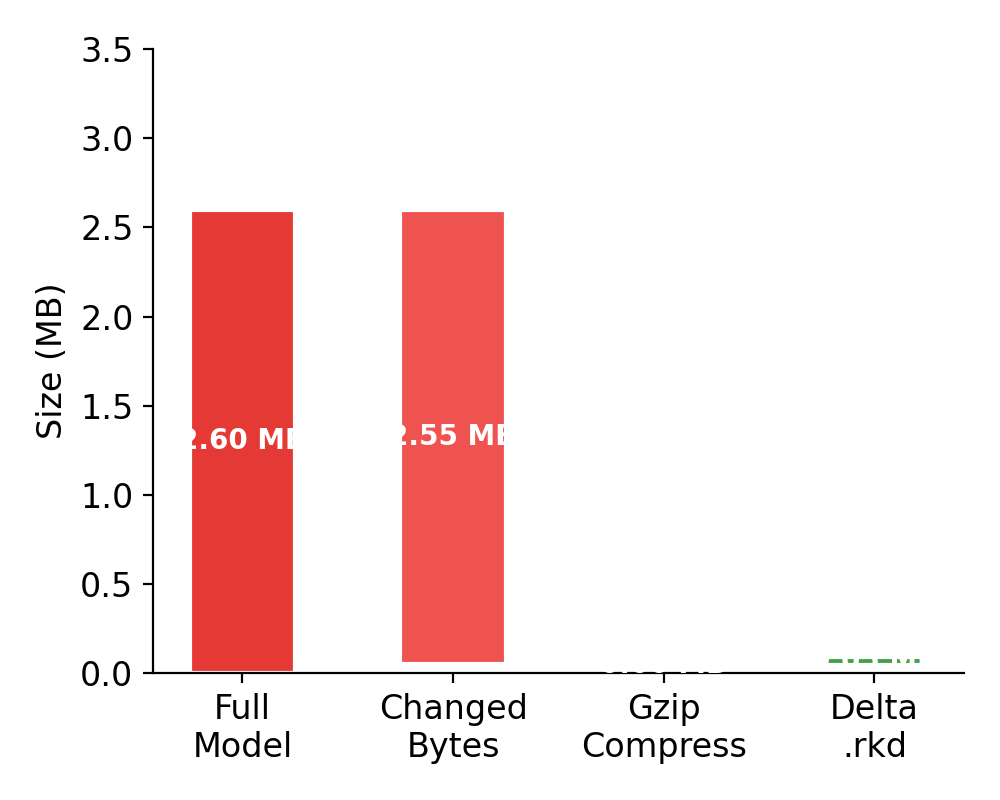
\includegraphics[width=\textwidth]{charts/delta_savings.png}
  \end{columns}
\end{frame}

% ── Slide 8: Telegram Bot ──
\begin{frame}{Telegram Bot --- Operasional Lapangan}
  \textbf{Bot self-hosted} untuk warga yang tidak menggunakan Android app.

  \vspace{0.2cm}
  \begin{columns}[T]
    \column{0.48\textwidth}
    \textbf{Fitur:}
    \begin{itemize}
      \item Kirim foto $\rightarrow$ ML langsung
      \item Kirim lokasi $\rightarrow$ analisis lingkungan
      \item Sequential flow (foto dulu / lokasi dulu)
      \item Laporan multifaktor lengkap
      \item Notifikasi admin kalo BAHAYA
    \end{itemize}

    \column{0.48\textwidth}
    \textbf{Teknis:}
    \begin{itemize}
      \item Python + python-telegram-bot
      \item Docker + uv build
      \item Polling mode (no SSL needed)
      \item Rate limited (10 req/60s)
      \item Supabase optional
    \end{itemize}
  \end{columns}
\end{frame}

% ── Slide 9: Progress ──
\begin{frame}{Progress \& Roadmap}
  \centering
  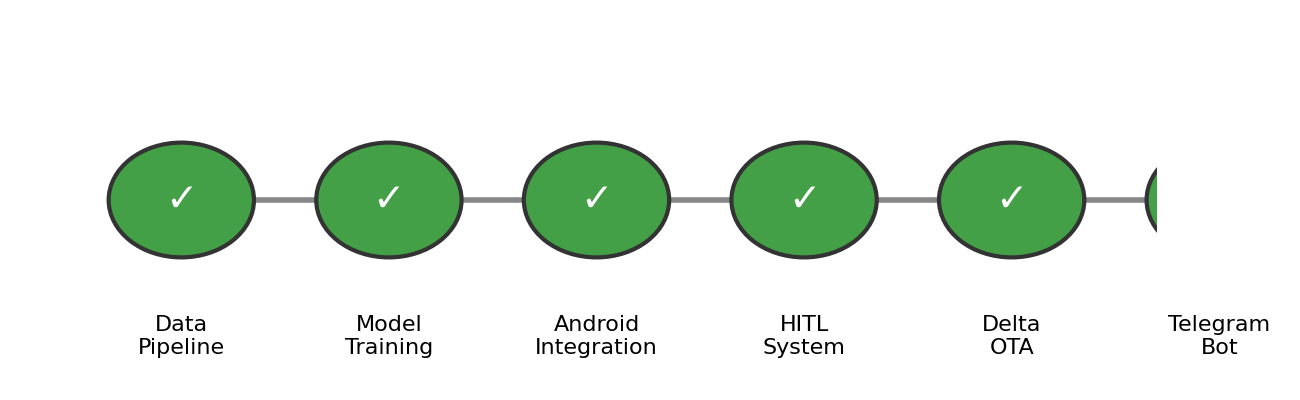
\includegraphics[width=0.85\textwidth]{charts/timeline.png}
  \vspace{0.3cm}

  \begin{columns}[T]
    \column{0.32\textwidth}
    \textbf{ Done}
    \begin{itemize}
      \tiny
      \item Data pipeline
      \item Model training v3a
      \item Android app
      \item Web app
      \item Multi-factor risk
      \item Telegram bot
      \item Delta OTA
    \end{itemize}

    \column{0.32\textwidth}
    \textbf{ In Progress}
    \begin{itemize}
      \tiny
      \item Deployment produksi
      \item Admin dashboard
      \item HITL loop
    \end{itemize}

    \column{0.32\textwidth}
    \textbf{ Next}
    \begin{itemize}
      \tiny
      \item Proximity alert
      \item Kearifan lokal
      \item Bimtek warga
    \end{itemize}
  \end{columns}
\end{frame}

% ── Slide 10: Thank You ──
\begin{frame}[standout]
  \textbf{Retak.id} \\
  \textit{One model, two platforms, zero excuses.} \\
  \vspace{0.5cm}
  \href{https://github.com/jaweed3/retakId}{\faGithub \space github.com/jaweed3/retakId}
\end{frame}

\end{document}
